% This is a default-selection of plugins that are used widely in this repo.

\documentclass[a4paper,10pt,fleqn]{article}
\usepackage[utf8]{inputenc}

% deutsche Trennmuster etc.
\usepackage[ngerman]{babel}
\usepackage[T1]{fontenc}

% mathematical simbols and fonts
\usepackage{mathtools} 
\usepackage{amssymb}
\usepackage{amsmath}
\usepackage{ntheorem}
\usepackage{polynom}
\usepackage{marvosym}
\usepackage{tabu}
\renewcommand*{\bmod}{\mathbin{\%}}
\everymath{\displaystyle}

\usepackage{multicol}
\usepackage{color}
\usepackage[usenames,dvipsnames]{xcolor}
\setlength{\columnsep}{1cm}
\setlength{\columnseprule}{0.25pt}
\def\columnseprulecolor{\color{gray}}
\usepackage{hyperref}

\usepackage[margin=1.5cm]{geometry}
\usepackage{graphicx}
\usepackage{pgfplots}
\pgfplotsset{compat=1.10}

%Code higlighting

\usepackage{minted}

% make lists more compact:
\newlength{\wideitemsep}
\setlength{\wideitemsep}{.5\itemsep}
\addtolength{\wideitemsep}{-5pt}
\let\olditem\item
\renewcommand{\item}{\setlength{\itemsep}{\wideitemsep}\olditem}
\renewcommand{\arraystretch}{1.25}

\title{Zusammenfassung An1I - Analysis 1 für Informatiker}
\author{Fabian Hauser}
 
\begin{document}
\maketitle
\begin{multicols}{2}
[
\section{Grundlagen}
]

\subsection{Mitternachtsformel}
	\[
		x_{1,2} = \frac{-b \pm\sqrt{b^2-4ac}}{2a}
	\]

\subsection{Mengen}
	Eine Menge ist eine Zusammenfassung verschiedener, voneinander unterscheidbarer Objekte zu einem Ganzen. Die Objekte nennen wir in diesem Zusammenhang auch die
	Elemente der Menge.

\subsubsection{Grundmengen}
	\begin{tabular}{l l}
		Reelen Zahlen & $\mathbb{R}=``\text{alle Zahlen}``$ \\
		Ganzen Zahlen & $\mathbb{Z}=\{\dots ,-1,0,1,2,\dots\}$ \\
		Natürliche Zahlen & $\mathbb{N}=\{0,1,2,\dots\}$ \\
		Leere Menge & $\emptyset = \{\}$
	\end{tabular}


\subsubsection{Elementbeziehungen}
	Die Elementbeziehungen dürfen Spiegelverkehrt verwendet werden.
	
	\begin{tabular}{l r}
		Element von & $a \in M$ \\
		kein Element von & $b \in M$ \\
		Teilmenge & $N \subset M$ \\
		keine Teilmenge & $K \not\subset M$ \\
		Gleichheit & $N = M$
	\end{tabular}

\subsubsection{Mengendarstellung}
	\begin{tabular}{l l}
		Aufzählend & $M = \{1,2,3\}$ \\
		Beschreibend & $M = \{x \in M|0<x<4\}$ \\
		Negative Teilmenge & $M^-= \{\dots\ ,-2,-1,0\}$ \\
		Positive Teilmenge & $M^+= \{0,1,2,\dots\}$
	\end{tabular}
	
	Die beschreibende Menge wird folgendermassen gelesen:
	\emph{Die Menge aller $x$ aus $M$ für die gilt: $0<x<4$} 
	
	Ein Filter darf als Prosa genannt werden, und muss auf alle Elemente anwendbar sein.

\subsubsection{Intervalle}
	\begin{align*}
		(1;200] = \{x \in\mathbb{R}|1<x \leq 200\} \\
		[1;200] = \{x\in\mathbb{R}|1\leq x \leq 200\}
	\end{align*}

\end{multicols}

\begin{multicols}{2}[
	\section{Funktionen}
]
	Eine Funktion hat immer einen oder mehrere Eingabe- und einen Ausgabewert. Für diese müssen Eingabe- und Ausgabemenge definiert werden, welche immer zutreffen.
	
	Für Elemente daraus ist die Funktion zwingend \emph{wohldefiniert}, d.h. vollständig Anwendbar auf alle Elemente der Eingabemenge. Die Zielmenge darf Werte enthalten, welche im Resultat nicht vorkommen (dies schränkt die Weiterverarbeitung ein.)
	
	Eine Funktion kennt \emph{keinen Zustand} (d.h. gleiche Eingabe $\Rightarrow$ gleiche Ausgabe).
	
	Funktionen können auch auf Mengen angewendet werden.
	
	Nur wenn alle obigen Bedingungen zutreffen, handelt es sich um eine Funktion. Um dies bei einer impliziten, d.h. in Prosa definierten Funktion festzustellen, muss diese in eine explizite Funktion umgewandelt werden.


\subsubsection{Definition}
	Gegeben seien zwei Mengen D und Z. Eine Zuordnungsvorschrift $f$, die jedem Element aus $D$ genau ein Element aus $Z$ zuordnet, nennen wir eine Funktion und schreiben dafür:
	\[
		\underbracket{
			\overbracket{f}^\text{Name} : \left\{
			\underbracket{
				\begin{array}{ll}
					\overbracket{
						\mathbb{R}^{\vphantom{+}} % vphantom just to adjust height, no mathematical meaning. ugly workaround.
					}^{
						\mathclap{
							\text{Definitionsmenge}
						}
					}
					& \to \overbracket{
						\mathbb{R}^+
					}^{
						\mathrlap{\!\text{Zielmenge}}
					} \\
					\underbracket{x}_{
						\mathclap{\!\text{Input}}
					}
					& \mapsto \underbracket{x^2}_{
						\mathclap{\!\text{Output}}
					}
				\end{array}
			}_\text{Transformationsvorschrift}
			\right.
		}_\text{Zuordnungsvorschrift}
	\]
	
	Um die Funktion anzuwenden, wird folgende Syntax verwendet:
	\[\overbracket{
		f(\underbracket{4}_{\mathrlap{\text{Funktionsargument}}})
	}^{\mathrlap{\text{Funktionswert (Zahl)}}}
	= 4^2 = 16
	\]
	
\subsubsection{Lösungsvorgehen}
	\begin{enumerate}
		\item Liegt 4 in Definitionsmenge
		\item Wenden Sie die Funktionsvorschrift auf Argument 4 an.
	\end{enumerate}

\subsubsection{Bild einer Funktion}
	Als das Bild einer Funktion wird die Menge aller möglichen Ergebnisse bezeichnet. Diese Menge lässt sich auf einem Graphen von der X-Achse auslesen.
	
	Beispiel: $f(\mathbb{R}) = \mathbb{R}^+$
	
\subsubsection{Graph einer Funktion}
	Als Graph von $f$ bezeichnet man die möglichen Wertepaare, für die es ein y = f(x) gibt:
	\[
		Graph(f) = \{(x,y) \in D \times Z | y=f(x)\}
	\]
	
	für die Funktion: 
	\[
		f:
		\begin{cases}
			D &\to Z \\
			x &\mapsto f(x)
		\end{cases}
	\]

\subsection{Elementare Funktionen ohne Trigonometrie}

\subsubsection{Potenzen}
	Sei $n \in \mathbb{N}\setminus\{0\}$:
	\[
		\cdot^n : \begin{cases}
			\mathbb{R} &\to \mathbb{R} \\
			x &\mapsto \underbrace{x \cdot x \cdot \ldots \cdot x}_\text{n Faktoren}
		\end{cases}
	\]
	
	Daraus folgt:
	\begin{align}
		a^n \cdot a^m &= a ^{n+m} \\
		\frac{a^n}{a^m} &= a^{n-m} \\
		a^{n \cdot m} &= (a^n)^m \\
		a^n \cdot b^n &= (a \cdot b)^n \\
		\frac{a^n}{b^n} &= (\frac{a}{b})^n \\
		a^{-n} &= \frac{1}{a^n} \\
		a^0 &= 1 \\
		a^1 &= a
	\end{align}

	Definitionen: \newline	
	(7) insbesondere gilt $0^0=1$, aber (8) $0^n=0$ \newline	
	(6) für $f\tilde{w} a \not= 0$

\subsubsection{Wurzeln}
	Sei $a>0$ und $m,n \in \mathbb{R}$:
	\[
		a^\frac{m}{n} = \sqrt[n]{a^m}
	\]

\subsubsection{Exponentialfunktion}
	
	Für $a>0$ gilt die folgende Definition:
	\[
		\exp_a : \begin{cases}
			\mathbb{R} &\to \mathbb{R^+}\setminus \{0\} \\
			x &\mapsto a^x
		\end{cases}
	\]	

	Die Exponentialfunktion ist eine gerade Funktion:
	$\sqrt{a^2} = \sqrt{\left|a\right|^2} = \left|a\right|$ für $a > 0$

	\paragraph{Wichtige Rechenregeln}
		\begin{align*}
			\exp_a{(x+y)} &= \exp_a{x} \cdot \exp_a{y} \\
			\exp_a{(x-y)} &= \frac{\exp_a{x}}{\exp_a{y}} \\
			(\exp_a{x})^y &= \exp_a{(x \cdot y)} \\
			\exp_a{-x} &= \frac{1}{\exp_a{x}}
		\end{align*}
	
\subsubsection{Wurzelfunktion}
	\[
		\sqrt{\cdot} : \begin{cases}
			\mathbb{R}^+ &\to \mathbb{R}^+ \\
			x & \mapsto \text{positive Lösung der Gleichung: $y^2=x$}
		\end{cases}
	\]

\subsubsection{Logarithmus}
	Sei $a,b > 0$: $a^x = b  \iff x = \log_a{b}$

	\[
		\log_a \cdot : \begin{cases}
			\mathbb{R}^+ \setminus \{0\} &\to \mathbb{R} \\
			y &\mapsto \text{Lösung der Gleichung } a^x = y
		\end{cases}
	\]

	\paragraph{Wichtige Rechenregeln}
		\begin{align*}
			\log_a{(x \cdot y)} &= \log_a{x} + log_a{y} \\
			\log_a{\frac{x}{y}} &= \log_a{x} - log_a{y} \\
			\log_a{(x^y)} &= y \cdot \log_a{x} \\ \\
			x=\log_a{y} &\Leftrightarrow a^{\log_a{y}} = y
		\end{align*}

\subsubsection{Natürlicher Logarithmus}
	Als Natürlicher Logarithmus wird die Funktion $\ln$ bezeichnet:
	\[
		\ln{x} = log_e{x}
	\]
	
\subsubsection{Umkehrfunktionen}
	
	\[
		f: \begin{cases}
			D &\to Z \\
			x &\mapsto f(x)
		\end{cases}
	\]
	
	\begin{description}
		\item[Surjektive Funktionen] \hfill \\
			$\text{Bild}(f) = Z$ \newline Die Zielwerte sing gleich der Zielmenge.
		\item[Injektive Funktionen] \hfill \\
			$\text{aus } x \neq y \text{ stehts } f(x) \neq f(y)$ \newline Es gibt für keinen Parameter die gleiche Rückgabe wie für einen anderen.
		\item[Bijektive Funktionen] \hfill \\
			Sind sowohl surjektiv als auch injektiv.
	\end{description}
	

	Wenn $f$ bijektiv ist, heisst die\newline Umkehrfunktion von $f$:
	\[
		\underbracket{f^{-1}}_{\mathclap{\text{Funktionsname\space\space\space\space\space\space}}} : \begin{cases}
			Z &\to D \\
			y &\mapsto \text{Lösung der Gleichung } f(x) = y
		\end{cases}
	\]
	
\subsubsection{Restriktion einer Funktion}

	Sei $f: D \to Z$ irgendeine Funktion, dann heisst die Restriktion von $f$ auf $M$
	\[
		f\mid_M : \begin{cases}
			M &\to Z \\
			x &\mapsto f(x)
		\end{cases}
	\]

\subsection{Gleichungen ohne Trigonometrie}

%TODO: Übertragen von "1.3.5. Regeln zum Umformen von Gleichungen. Die in Abschnitt 1.3.3 beschriebenen", s. 57

\subsubsection{Äquivalenzumformungen}
	Änderungen welche am Wahrheitsgehalt nichts ändern. Dies wird ausgedrückt durch: $\Leftrightarrow$
	
	Wenn einer Umwandlung eine Einschränkung oder Bedingung auferlegt wird, so wird dies durch eine Bezeichnung auf dem $\Leftrightarrow$ dargestellt: $\xLeftrightarrow{x \neq 0 \text{, sonst unlösbar}}$
	Resultate müssen immer gegen diese Bedingung(en) geprüft werden.
	Bei Bedingungen ergibt sich immer ein Sondergfall, welcher explizit abgehandelt werden muss (Text nach Bedingung).
	
	Es dürfen nur injektive Funktionen auf beide Seiten angewendet werden, wenn beide Werte im Definitionsbereich sind. Dies muss allerdings dargestellt werden: $\xLeftrightarrow{\text{T}_1(x), \text{T}_2(x) \in \text{DB}_f \mathrlap{\text{, sonst unlösbar}}}$
	
	Bei nicht-injektive Funktionen kann nur einseitig gefolgert werden ($\Rightarrow$). Oft können Funktionen (z.B. $\cdot^2$) injektiv gemacht werden, indem sie eingeschränkt definiert werden (z.B. $\cdot^2_{|\mathbb{R}^+}$)
	
\subsection{Trigonometrische Funktionen}
	
	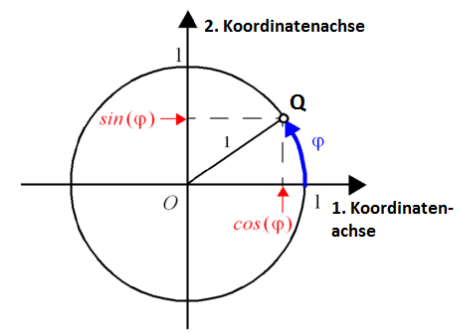
\includegraphics[scale=0.33]{img/einheitskreis_sin_cos.png}
	
\subsubsection{Fundamentale Beziehungen}

	\begin{align*}
		\tan(\alpha) &= \frac{\sin \alpha}{\cos \alpha} & \text{für } \cos(\alpha) \neq 0 \\
		\cos(x) &= \tan(x) \cdot \sin(x) \\ %TODO: ?
		 1 &=  \sin^2(\alpha) + \cos^2(\alpha) \\
		 -\cos(\alpha) &= \cos(\pi - \alpha) \\
		 \sin(\alpha) &= \sin(\pi - \alpha)
	\end{align*}
	
\subsubsection{Umkehrfunktion Cosinus}

	Der Cosinus ist nicht injektiv, da er nach $\frac{\pi}{2}$ immer die gleichen $y$-Werte liefert. Daher ist eine Einschränkung nötig:
	$\cos|_{[0;\pi]}$
	\[
		arccos : \begin{cases}
			[-1, -1] &\to [0;\pi]\\tablular
			y &\mapsto \text{Lösung } x \in [0;\pi] \text{ der}\\
			  &\indent \text{Gleichung }  cos(x) = y
		\end{cases}
	\]tablular
	
	Aufgrund der repetitiven sowie nicht injektiven tablularEigenschaft des Cosinus lässt sich daraus folgendes festlegen:
	\[
		cos(x) = y \iff x = \pm \arccos(y) + 2 \pi k, k \in \mathbb{Z}
	\]
	
\subsubsection{Umkehrfunktion Sinus}
	tablular
	Der Sinus ist nicht injektiv, da er nach $\frac{\pi}{2}$ immer die gleichen $y$-Werte liefert. Daher ist eine Einschränkung nötig:
	$\sin|_{[-\frac{\pi}{2};\frac{\pi}{2}]}$
	
	\[
		arcsin : \begin{cases}
			[-1;1] &\to [-\frac{\pi}{2};\frac{\pi}{2}]\\
			y &\mapsto \text{Lösung } x \in [-\frac{\pi}{2};\frac{\pi}{2}]\\
			  &\indent \text{ der Gleichung } sin(x)=y
		\end{cases}
	\]
	
	
	Daraus lässt sich folgende konkrete Anwendung herleiten:
	
	\[
		y = sin(x) \iff x = \begin{cases}
			\arcsin(y) + 2 \pi k, k \in \mathbb{Z}\\
			\pi - \arcsin(y) + 2 \pi k, k \in \mathbb{Z}
		\end{cases}
	\]
	
\subsubsection{Umkehrfunktion Tangens}
	
	Der Tangens ist nicht injektiv, deshalb: $\tan|_{(\frac{\pi}{2}; \frac{\pi}{2})}$
	
	Daraus lässt sich folgern:
	
	\[
		y = tan(x) \iff x = \arctan(y) + \pi k, k \in \mathbb{Z}
	\]
	
%TODO: Seite 74|1.5.4 und 75|1.6 ergänzen

\subsection{Ungleichungen}

\begin{tabular}{l l}
	Monoton wachsend & $x_1 < x_2 \iff f(x_1) < f(x_2)$ \\
	Monoton fallend & $x_1 < x_2 \iff f(x_1) > f(x_2)$
\end{tabular}

\end{multicols}

\section{Differenzialrechnung}

\subsection{Splines}

	Splines werden durch Polynome zwischen zwei Punkten abgebildet.	Splines bilden alle diese Punkte exakt ab.
	
	Ein Spline im Intervall $[a,b]$ ist eine Funktion $s: [a,b] \to \mathbb{R}$, wofür es $k+1$ Knoten (typischerweise x-Achse) gibt:
	\[
	a = x_0 < x_1 < x_2 < ... < x_k = b
	\]
	
	$s|_{[x_i;x_{i+1}]}$ ist stets ein Polynom $n$ter Ordnung, daher gilt: $s|_{[x_i;x_{i+1}]}(x) = P_k(x)$
	
	Ein Spline vom Grad $n$ heisst: Alle Polynome sind $\leq n$ter Ordnung
	
	\subsubsection{Beispiel Spline 1. Grad}
	
	\begin{align*}
		P_k(x) = mx_k \cdot b_k \\
		m \cdot x_k + b_k &= s \\
		m \cdot x_{k+1} + b &= s_{k + 1}
	\end{align*}
\end{document}